\documentclass[letter,12pt]{article}
\usepackage[paperheight=27.94cm,paperwidth=21.59cm,bindingoffset=0in,left=3cm,right=2.0cm, top=3.5cm,bottom=2.5cm, headheight=200pt, headsep=1.0\baselineskip]{geometry}
\usepackage{graphicx,lastpage}
\usepackage{upgreek}
\usepackage{censor}
\usepackage[spanish,es-tabla]{babel}
\usepackage{pdfpages}
\usepackage{tabularx}
\usepackage{graphicx}
\usepackage{adjustbox}
\usepackage{colortbl}
\usepackage{rotating}
\usepackage{multirow}
\usepackage[utf8]{inputenc}
\usepackage{float}
\usepackage{hyperref}

% CUSTOM %
\definecolor{backcolour}{rgb}{0.95,0.95,0.92}
\definecolor{codegreen}{rgb}{0,0.6,0}
\definecolor{codegray}{rgb}{0.5,0.5,0.5}
\definecolor{codepurple}{rgb}{0.58,0,0.82}

\usepackage[most]{tcolorbox}
\usepackage{listings}
\usepackage{xcolor}



\definecolor{myyellow}{RGB}{255, 255, 204}

\lstdefinestyle{mystyle}{
	backgroundcolor=\color{backcolour},
	commentstyle=\color{codegreen},
	keywordstyle=\color{magenta},
	numberstyle=\tiny\color{codegray},
	stringstyle=\color{codepurple},
	basicstyle=\ttfamily\footnotesize,
	breakatwhitespace=false,         
	breaklines=true,                 
	captionpos=b,                    
	keepspaces=true,                 
	numbers=left,                    
	numbersep=5pt,                  
	showspaces=false,                
	showstringspaces=false,
	showtabs=false,                  
	tabsize=2
}

%"mystyle" code listing set
\lstset{style=mystyle}

% END CUSTOM%
\renewcommand{\tablename}{Tabla}
\usepackage{fancyhdr}
\pagestyle{fancy}


%
\begin{document}
%
   \title{\Huge{Informe Laboratorio 1}}

   \author{\textbf{Sección X} \\  \\Alumno X \\ e-mail: alumno.contacto@mail.udp.cl}
          
   \date{Marzo de 2024}

   \maketitle
   
   \tableofcontents
 
  \newpage
  

\section{Descripción}

\begin{enumerate}
    \item Usted empieza a trabajar en una empresa tecnológica que se jacta de poseer sistemas que permiten identificar filtraciones de información a través de Deep Packet Inspection (DPI).\\
    A usted le han encomendado auditar si efectivamente estos sistemas son capaces de detectar las filtraciones a través de tráfico de red. Debido a que el programa ping es ampliamente utilizado desde dentro y hacia fuera de la empresa, su tarea será crear un software que permita replicar tráfico generado por el programa ping con su configuración por defecto, pero con fragmentos de información confidencial. Recuerde que al comparar tráfico real con el generado no debe gatillar alarmas. \\
    De todas formas, deberá hacer una prueba de concepto, en la cual se demuestre que al conocer el algoritmo, será fácil determinar el mensaje en claro.
    


\end{enumerate}


\section{Actividades}


\subsection{Algoritmo de cifrado}

\begin{enumerate}
\item Generar un programa, en python3, que permita cifrar texto utilizando el algoritmo Cesar. Como parámetros de su programa deberá ingresar el string a cifrar y luego el corrimiento.
\begin{figure}[H]
        \centering
        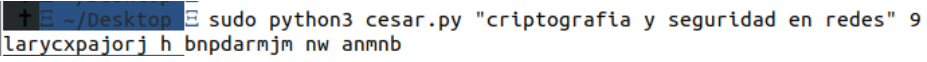
\includegraphics[width=15cm]{actividades/A1.png}
        \label{fig:a1}
\end{figure}


\end{enumerate}

\subsection{Modo stealth}

\begin{enumerate}
    \item Generar un programa, en python3, que permita enviar los caracteres del string (el del paso 1) en varios paquetes ICMP request (un caracter por paquete en el byte menos significativo del contador ubicado en el campo data de ICMP) para que de esta forma no se gatillen sospechas sobre la filtración de datos.\\
    Para la generación del tráfico ICMP, deberá basarse en los campos de un paquete generado por el programa ping basado en Ubuntu, según lo visto en el lab anterior disponible \href{https://www.cloudshark.org/captures/d5b420cd47de}{acá}.\\
    El envío deberá poder enviarse a cualquier IP. Para no generar tráfico malicioso dentro de esta experiencia, se debe enviar el tráfico a la IP de loopback.\\
    \begin{figure}[H]
        \centering
        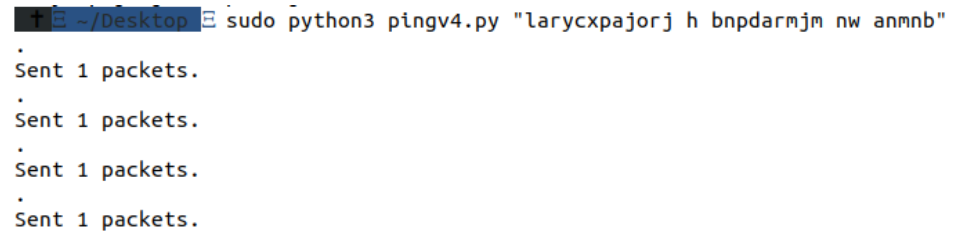
\includegraphics[width=15cm]{actividades/A2.1.png}
        \label{fig:a2-1}
    \end{figure}
    A modo de ejemplo, en este caso, cada paquete transmite un caracter, donde el último paquete transmite la letra b, correspondiente al caracter en plano \textquotedblleft s\textquotedblright.
    \begin{figure}[H]
            \centering
            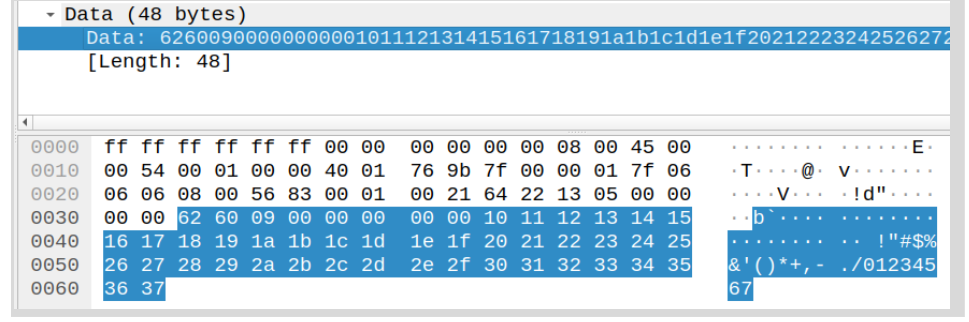
\includegraphics[width=15cm]{actividades/A2.2.png}
            \label{fig:a2-2}
        \end{figure}
\end{enumerate}

\clearpage

\subsection{MitM}
\begin{enumerate}
    \item Generar un programa, en python3, que permita obtener el mensaje transmitido en el paso2. Como no se sabe cual es el corrimiento utilizado, genere todas las combinaciones posibles e imprímalas, indicando en verde la opción más probable de ser el mensaje en claro.
    \begin{figure}[H]
        \centering
        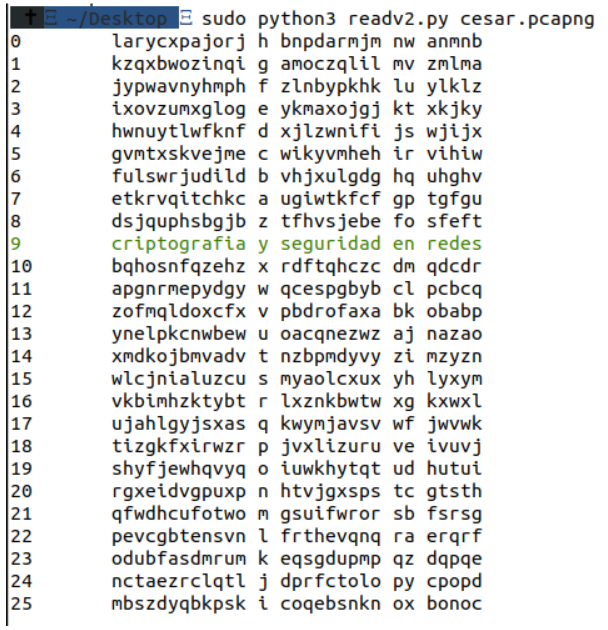
\includegraphics[width=12cm]{actividades/A3.png}
        \label{fig:a3}
    \end{figure}
    Finalmente, deberá indicar los 4 mayores problemas o complicaciones que usted tuvo durante el proceso del laboratorio y de qué forma los solucionó.

\end{enumerate}

\section{Desarrollo de Actividades}

\subsection{Actividad 1}

\subsection{Actividad 2}

\subsection{Actividad 3}

\section*{Conclusiones y Comentarios}

\subsection*{Issues}

\end{document}
